%----------------------------------------------------------------------------------------
%	PACKAGES AND OTHER DOCUMENT CONFIGURATIONS
%----------------------------------------------------------------------------------------

\documentclass[a4paper,11pt]{article} % Font and paper size

%----------------------------------------------------------------------------------------
%	PACKAGES AND OTHER DOCUMENT CONFIGURATIONS
%----------------------------------------------------------------------------------------

\usepackage[utf8]{inputenc} % Required for inputting international characters
\usepackage[T1]{fontenc} % Output font encoding for international characters
\usepackage[italian]{babel} % Italian dictionary


\usepackage[table]{xcolor} % Required for custom colors
\usepackage{gensymb}
\usepackage{amsmath}
\usepackage{bm}
\usepackage{tikz}
\usepackage{hhline}
\usepackage{listings}
\usepackage{enumitem}

%\usepackage[margin=2cm, includefoot]{geometry} % Modify margins
\usepackage{fancyhdr}
\usepackage{rotating}
\usepackage[hidelinks]{hyperref} % Hyperlinks

\usepackage[none]{hyphenat}% Non spezza le parole nelle tabelle
\usepackage{array}

\usepackage{graphicx} % Required for figures
\usepackage{float}
\usepackage{wrapfig}
\usepackage{caption}
\usepackage{subcaption}

%pagestyle
\pagestyle{fancy}
\fancyhead{}
\fancyfoot{}
\fancyfoot[R]{\thepage}
\renewcommand{\headrulewidth}{0pt}



\usepackage{xfrac}
\usepackage{amssymb}

\usepackage{multicol}
\usepackage{multirow}

\usepackage[toc, page]{appendix}
\usepackage{booktabs}
\usepackage{siunitx}


%----------------------------------------------------------------------------------------
%	NEW COMMANDS
%----------------------------------------------------------------------------------------

\newcommand{\restr}[2]{{% we make the whole thing an ordinary symbol
\left.\kern-\nulldelimiterspace % automatically resize the bar with \right
#1 % the function

\right|_{#2} % this is the delimiter
}}

\newcommand{\tnhl}{\tabularnewline\hline}
\newcommand{\tn}{\tabularnewline}
\newcolumntype{x}[1]{%
	>{\centering\hspace{0pt}}p{#1}}%


 % Include the file specifying document layout and packages


%----------------------------------------------------------------------------------------
%	GENERAL INFORMATION 
%----------------------------------------------------------------------------------------

\newcommand{\labcourse}{Laboratorio di Fisica}
\newcommand{\teacher}{Docenti: Prof. A. Garfagnini - Prof. M. Lunardon}
\newcommand{\laurea}{Corso di Laurea in Fisica}
\newcommand{\channel}{Canale 1 A-L}
\newcommand{\academicyear}{Anno Accademico 2020/2021}
\newcommand{\labexp}{Esperienza di Laboratorio}
\newcommand{\exptitle}{Amplificatori Operazionali \& Calibrazione Arduino}
\newcommand{\turno}{Turno T2}
\newcommand{\name}{Nicolò Lai}
\newcommand{\matricola}{1193976}
\newcommand{\mail}{nicolo.lai@studenti.unipd.it}
\newcommand{\consegna}{Data Esperienza}
\newcommand{\data}{28/10/2020 - 29/10/2020}


%----------------------------------------------------------------------------------------
%	DOCUMENT 
%----------------------------------------------------------------------------------------

\begin{document}

%----------------------------------------------------------------------------------------
%	REFERNCE CUSTOMIZATION
%----------------------------------------------------------------------------------------

\def\sectionautorefname{Sezione} 
\def\subsectionautorefname{Sezione} 
\def\subsubsectionautorefname{Sezione}

%----------------------------------------------------------------------------------------
%	TITLE PAGE
%----------------------------------------------------------------------------------------

\begin{titlepage}
	\begin{center}
		\Huge{\bfseries \labcourse}\\
			
		\LARGE \teacher \\
		\Large \laurea\\
		\Large \channel\\
		\Large \academicyear\\
		[1cm] 
		\line(1,0){400}\\
		[3.5cm]
			
		\textsc{\huge{\bfseries \labexp}}\\
		\huge{\exptitle}\\
		[2mm] \line(1,0){300}\\
		[10cm]
	\end{center}
	
	
	\begin{flushleft}
		\textsc{\Large \turno}\\
		[0.5cm] \textsc{\large {\bfseries \name}} \\ 
		\indent\large \matricola \\ 
		\indent\large \mail \\
	\end{flushleft}
		
					
	\begin{flushright}
			\textsc{\Large\consegna}\\
			\textsc{\large \data}					
	\end{flushright}
			
\end{titlepage}
\cleardoublepage


%----------------------------------------------------------------------------------------
%	OBIETTIVO
%----------------------------------------------------------------------------------------

\section{Obiettivo}
Verificare la linearità di un amplificatore operazionale e misurare l'amplificazione di un circuito che lo comprenda.
Misurare la frequenza di taglio di un filtro attivo. Calcolare il sampling rate e la funzione di calibrazione in
tensione di una scheda Arduino Due.

%----------------------------------------------------------------------------------------
%	APPARATO SPERIMENTALE
%----------------------------------------------------------------------------------------

\section{Strumentazione e Componenti}\label{s:strumenti}
Nel corso dell'esperienza si utilizzano i seguenti:
\begin{itemize}
	\item Multimetro digitale Metrix MTX3292
	\item Generatore di funzioni Tektronix AFG1022
	\item Oscilloscopio digitale Tektronix TBS1102B
	\item Alimentatore di tensione continua TTi
	\item Circuito integrato TL082C (contenente due amplificatori operazionali)
	\item Tre resistori $R_{\text{f}}$, $R_{1}$, $R_{3}$ ed un condensatore $C_{1}$ 
	\item Scheda Arduino Due
\end{itemize}

%\begin{itemize}
%	\item \textbf{Oscilloscopio} (Tektronix TBS1102B): Lo strumento presenta un'accuratezza sul guadagno verticale $\Delta_{g}$ pari
%	al 3\% del valore letto (errore massimo) ed è \textit{generalmente} il contributo più significativo. L'incertezza di
%	guadagno sui tempi si assume trascurabile. L'accuratezza che tiene conto degli effetti di risoluzione e imprecisione
%	della traccia $\Delta_{l}$ è di 1/10 di divisione su tutta la scala di lettura (errore massimo), uguale sia per le tensioni sia
%	per i tempi.
%
%	\item \textbf{Generatore di funzioni} (Tektronix AFG1022)
%
%	\item  \textbf{Alimentatore di tensione continua}: Lo strumento presenta due uscite con erogazione di tensione tra 0
%	e 20 \si{\volt} e un'uscita con erogazione fissata a 5 \si{\volt}
%	
%	\item \textbf{Multimetro digitale} (Metrix MTX3292): Si riporta l'accuratezza dello strumento, per misure di
%	resistenza e di capacità, relativa unicamente ai fondoscala utilizzati nell'esperienza.
%
%	\begin{table}[H]
%		\small
%		\centering
%		\begin{tabular}{x{2cm} x{3cm} x{3cm} } \toprule[0.5px]\toprule[0.1px]
%			
%			\multicolumn{3}{c}{Accuratezza Metrix MTX3292}\tn
%			\midrule[0.1px]
%			
%			F.S. & Precisione & Risoluzione \tn
%			
%			\addlinespace
%			
%			1   \si{k\ohm} & 0.10\% + 8  & 0.01 \si{\ohm}  \tn 10  \si{k\ohm} & 0.07\% + 8  & 0.1  \si{\ohm}  \tn 100
%			\si{k\ohm} & 0.07\% + 8  & 1 \si{\ohm}  \tn
%
%			
%			\addlinespace
%
%			1000 \si{p\farad}         & 2.5\% + 15  & 1 \si{p\farad}   \tn
%			
%			\bottomrule[0.5px]
%			
%			
%		\end{tabular}
%		\caption{Per i fondoscala indicati si riportano la precisione (contributo di scala in percentuale e contributo
%		di lettura sul digit meno significativo) e la risoluzione dello strumento.}
%		\label{t:metrix}
%	\end{table}	 
%
%	\item \textbf{Componenti circuitali} (Resistori e Condensatori): Si riportano i valori delle resistenze e capacità
%	utilizzate per l'assemblamento dei circuiti utilizzati nel corso dell'esperienza, misurate preliminarmente con il
%	multimetro digitale Metrix. 
%
%	\begin{table}[H]
%		\small
%		\centering
%		\begin{tabular}{x{2cm} x{3cm} x{3cm} } \toprule[0.5px]\toprule[0.1px]
%			
%			\multicolumn{3}{c}{Resistori e Condensatori}\tn
%			\midrule[0.1px]
%			
%			Resistenza & Valore & F.S. \tn
%			
%			\addlinespace
%			
%			$R_{\text{f}}$ & $(82.46 \pm 0.03)\,\si{k\ohm}$ & $100\,\si{k\ohm}$ \tn
%
%			$R_1$ & $(8.089 \pm 0.003)\,\si{k\ohm}$ & $10\,\si{k\ohm}$ \tn
%
%			$R_3$ & $(46.54 \pm 0.05)\,\si{\ohm}$ & $1\,\si{k\ohm}$ \tn
%		
%			\addlinespace
%
%			\midrule[0.1px]
%			
%			Capacità & Valore & F.S. \tn
%			
%			\addlinespace
%
%			$C_1$  & $(977 \pm 17)\,\si{p\farad}$  & $1000\,\si{p\farad}$   \tn
%			
%			\bottomrule[0.5px]
%			
%		\end{tabular}
%		\caption{In tabella si indicano le componenti circuitali (resistori e capacità) utilizzando delle label
%		specifiche per ciascuna di esse: questa notazione è costante nel corso dell'esperienza.}
%		\label{t:direct_measures}
%	\end{table}	
%
%	\item \textbf{Circuito integrato TL082C} (Due Amplificatori Operazionali): essendo gli amplificatori operazionali
%	delle componenti circuitali attive, esse devono essere alimentate. Si utilizza dunque il generatore di tensione
%	continua con $V_{\text{cc}} = +15\,\si{\volt}$ e $V_{\text{ee}}=-15\,\si{\volt}$ per l'alimentazione
%	dell'amplificatore operazionale utilizzato nell'esperienza. Nel corso di quest'ultima, si assume un comportamento
%	\textit{ideale} dell'amplificatore operazionale, ovvero che il polo positivo ed il polo negativo si trovino
%	allo stesso potenziale.
%	
%	\item \textbf{Scheda Arduino Due}
%\end{itemize}


%----------------------------------------------------------------------------------------
%	AMPLIFICATORE OPERAZIONALE INVERTENTE
%----------------------------------------------------------------------------------------

\section{Amplificatore Operazionale Invertente}\label{s:opamp}
In questa sezione ci si propone di studiare il comportamento di un circuito puramente resistivo comprendente un
amplificatore operazionale in configurazione invertente (polo positivo a massa, polo negativo collegato al segnale in
ingresso). Si vuole in particolare verificare la sua linearità e stimare l'amplificazione del circuito come grandezza
derivata sia partendo dalle misure dirette delle resistenze sia come parametro di un'interpolazione lineare di misure
acquisite con l'oscilloscopio. 


%----------------------------------------------------------------------------------------
%	CONFIGURAZIONE SPERIMENTALE
%----------------------------------------------------------------------------------------

\subsection{Configurazione Sperimentale}\label{s:guadagno}

Si inizia assemblando il circuito, rappresentato in \autoref{i:opamp_circuit}, utilizzando le resistenze $R_{\text{f}}$, $R_1$,
$R_3$ e l'amplificatore operazionale. La resistenza $R_{\text{g}}$ rappresenta la resistenza interna del generatore, non nulla in
quanto ci si trova in condizioni di non idealità. Le resistenze esterne, invece, vengono misurate

\begin{wrapfigure}{R}{0.6\textwidth}
	\centering
	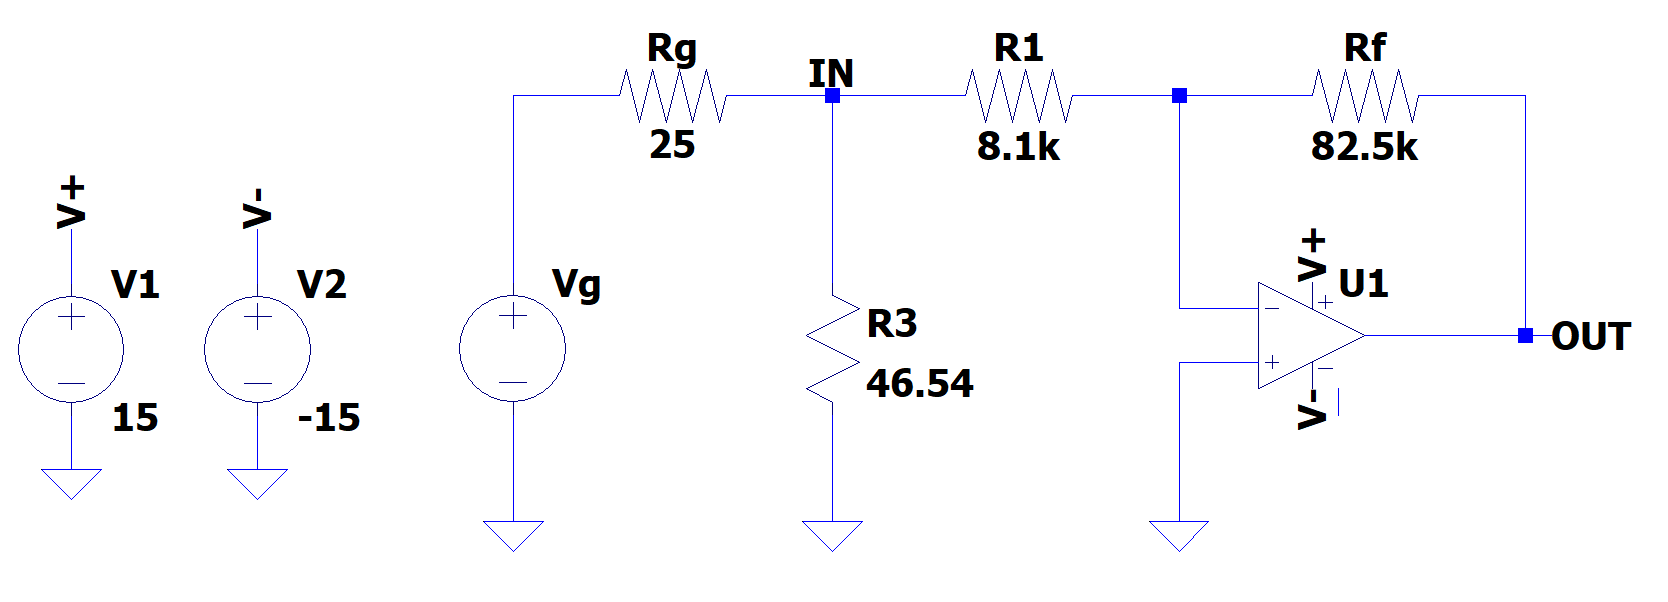
\includegraphics[width=0.6\textwidth]{../Simulations/OpAmp/circuit_image_nosim.png}
	\caption{\footnotesize Rappresentazione a variabili concentrate del circuito assemblato in laboratorio.}
	\label{i:opamp_circuit}
\end{wrapfigure}

\noindent direttamente utilizzando il multimetro Metrix MTX3292, ottenendo i risultati esposti in
\autoref{t:direct_measures}. Si utilizza poi un generatore di tensione continua con $V_{\text{cc}}=+15\,\si{\volt}$ e
$V_{\text{ee}}=-15\,\si{\volt}$ per l'alimentazione dell'amplificatore operazionale. Si assume, inoltre, che esso abbia
un comportamento ideale, ovvero che il polo positivo ed il polo negativo si trovino allo stesso potenziale. Il segnale
viene prelevato nei punti \textit{IN} e \textit{OUT} evidenziati nello schema in \autoref{i:opamp_circuit} (e verrà in
seguito richiamato rispettivamente come $V_{\text{in}}$ e $V_{\text{out}}$) utilizzando due sonde con fattore di
attenuazione 10X. Nel canale CH1 dell'oscilloscopio viene visualizzato il segnale in ingresso $V_{\text{in}}$, mentre il
segnale in uscita $V_{\text{out}}$ è prelevato dalla sonda collegata al canale CH2. Per entrambi i canali viene
selezionata la modalità "attenuazione sonda 10X", in modo da compensare la riduzione del segnale dovuta alle sonde e
visualizzare quindi nel display il segnale reale. Il generatore di funzioni viene poi configurato in

\begin{wraptable}{L}{0.5\textwidth}
	\small
	\centering
	\begin{tabular}{x{1.8cm} x{2.5cm} x{2cm} } \toprule[0.5px]\toprule[0.1px]
		
		\multicolumn{3}{c}{Misure Dirette delle Resistenze}\tn
		\midrule[0.1px]
		
		Resistenza & Valore & F.S. \tn
		
		\addlinespace
		
		$R_{\text{f}}$ & $82.46 \pm 0.03\,\si{k\ohm}$ & $100\,\si{k\ohm}$ \tn

		$R_1$ & $8.089 \pm 0.003\,\si{k\ohm}$ & $10\,\si{k\ohm}$ \tn

		$R_3$ & $46.54 \pm 0.05\,\si{\ohm}$ & $1\,\si{k\ohm}$ \tn
		
		\bottomrule[0.5px]		
	\end{tabular}
	\caption{\footnotesize Valori di resistenza, misurati direttamente con il multimetro, e relativo fondoscala.}
	\label{t:direct_measures}
\end{wraptable}	

\noindent  modalità "50 Ohm", in modo che l'impedenza d'uscita del generatore sia comparabile con
$R_3\approx 50\,\si{\ohm}$. Ci si aspetta così di trovare una tensione in ingresso $V_{\text{in}}$ in accordo con la
tensione nominale erogata dal generatore. Si imposta infine il generatore di funzioni in modo da erogare un segnale di
tipo sinusoidale con frequenza $f_{\text{gen}}=1\,\si{k\hertz}$, mantenuta costante in questa sezione, e di ampiezza
invece variabile tra $200\,\si{\mV}$ picco picco e $3.5\,\si{\V}$ picco picco. \\

\noindent Facendo riferimento ai valori delle resistenze $R_{\text{f}}$ ed $R_1$ riportate in \autoref{t:direct_measures}, si
vuole calcolare il guadagno $G$ del circuito atteso utilizzando l'\autoref{e:guadagno}, ottenuta risolvendo il circuito.
Si vuole far notare che, avendo posto l'amplificatore operazionale in configurazione invertente, si ritrova un segno
meno ad indicare un segnale in uscita $V_{\text{out}}$ "invertito" (ovvero ci si aspetta che i massimi del segnale in
ingresso corrispondano a minimi del segnale in uscita e viceversa). Tuttavia, nell'analisi che segue, verrà sempre
considerato il valore assoluto dell'amplificazione $G$, che si definisce dunque come
\begin{align}\label{e:guadagno}
	G&=\left|-\frac{R_{\text{f}}}{R_{1}}\right| = 10.194
	&
	\sigma_{G}&=\sqrt{	\left(	\frac{	1	}{	R_{1}	}	\right)^2	\sigma_{R_{\text{f}}}^2	
	+	\left(	\frac{	R_{\text{f}}	}{	R_{1}^2	}	\right)^2\sigma_{R_{1}}^2	}	= 0.006
\end{align}


%----------------------------------------------------------------------------------------
%	ACQUISIZIONE MISURE
%----------------------------------------------------------------------------------------

\subsection{Acquisizione Misure}
Al fine di verificare la linearità dell'amplificatore operazionale e stimare l'amplificazione del circuito, si decide di
far variare la tensione in ingresso impostando valori crescenti di ampiezza del segnale erogato dal generatore di
funzioni, partendo da $200\,\si{\mV}$ picco picco fino a $3.5\,\si{\V}$ picco picco. Per ciascuno di questi valori di
tensione si acquisisce la misura di un massimo e di un minimo sia del segnale $V_{\text{in}}$ sia del segnale
$V_{\text{out}}$ sfruttando i cursori orizzontali dell'oscilloscopio. In questo modo, si ottiene un campione di coppie
($V_{\text{in}}$, $V_{\text{out}}$) che ci si aspetta segua un andamento lineare, in quanto legate da
$V_{\text{out}}=-\frac{R_{\text{f}}}{R_{1}}V_{\text{in}}$ dove il segno meno, si ricorda, è dovuto all'operazionale
posto in configurazione invertente. Le misure in questione sono rappresentate in \autoref{i:opamp_eda}.


%----------------------------------------------------------------------------------------
%	SIMULAZIONE SPICE PRELIMINARE
%----------------------------------------------------------------------------------------

\subsection{Simulazione Spice Preliminare}\label{s:spice} Prima di procedere con l'analisi dati, si decide di simulare
la risposta del circuito utilizzando il software LTSpice. Vengono simulate due ampiezze in ingresso significative:
$V_{\text{gen}}=1\,\si{\volt}$ e $V_{\text{gen}}=4\,\si{\volt}$. 

\begin{wrapfigure}{L}{0.5\textwidth}
	\centering
	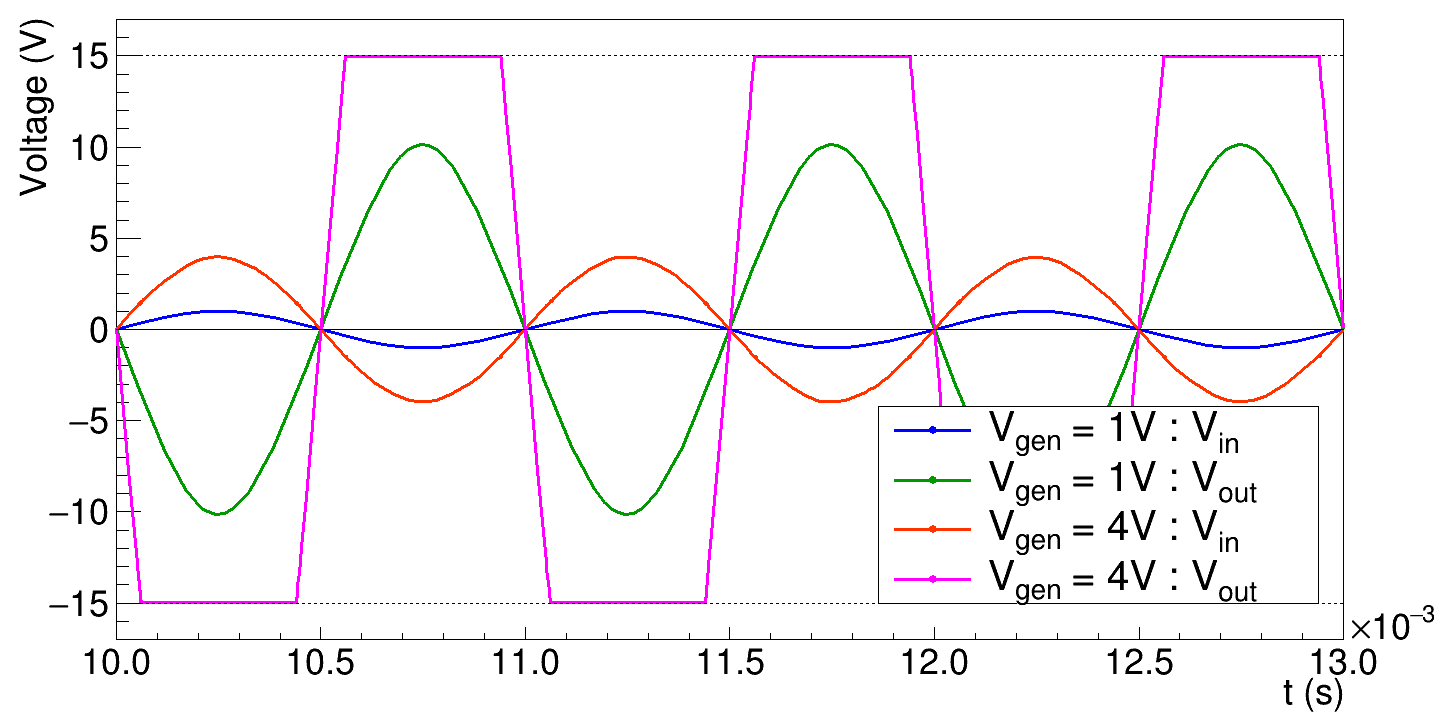
\includegraphics[width=0.5\textwidth]{../Plots/Report_Plots/opamp_spice_1V_4V_BIG.png}
	\caption{\footnotesize Simulazione Spice della risposta del circuito.}
	\label{i:opamp_simulation}
\end{wrapfigure}

\noindent L'amplificatore operazionale, essendo esso una componente attiva del circuito, non può fornire in output una
tensione maggiore di quanta ne riceve in alimentazione (per conservazione dell'energia): ci si aspetta allora di trovare
una situazione di saturazione del segnale in uscita e che questa inizi a manifestarsi attorno ad un valore nominale di
tensione $V\text{pp}_{\text{gen}}=3\,\si{\volt}$ in quanto, avendo un guadagno di circa 10, il segnale in uscita non può
superare i $30\,\si{\volt}$ picco picco. Dal grafico si evince chiaramente come erogando $V_{\text{gen}}=1\,\si{\volt}$
il segnale viene amplificato correttamente mantenendo la forma sinusoidale, mentre erogando
$V_{\text{gen}}=4\,\si{\volt}$ il segnale in uscita presenta i picchi tagliati esattamente a livello $V_{\text{sat}}=\pm
15\,\si{\volt}$, cioè le tensioni di alimentazione fornite all'operazionale. Inoltre, come anticipato in
\autoref{s:guadagno}, si può osservare il comportamento invertente dell'amplificatore operazionale.


%----------------------------------------------------------------------------------------
%	DATI E ANALISI
%----------------------------------------------------------------------------------------

\subsection{Dati e Analisi}
In questa sezione si vuole inizialmente rappresentare le misure acquisite in laboratorio riportandole in un grafico
esplorativo di $V_{\text{out}}$ contro $V_{\text{in}}$, per cercare di estrarre informazioni di carattere generale sui
dati a disposizione: per ogni misura di un massimo di $V_{\text{in}}$ si associa il corrispettivo massimo di
$V_{\text{out}}$ (analogo per i minimi). Successivamente, si vuole invece caratterizzare la linearità dell'amplificatore
operazionale ed il guadagno del circuito in termini statistici, focalizzandosi sullo studio di interpolazioni lineari.
Rappresentando in un grafico $V_{\text{out}}$ contro $V_{\text{in}}$, infatti, è possibile ricavare il valore assoluto
dell'amplificazione come il coefficiente angolare di una retta che interpola i dati: dalla bontà del fit e
dall'andamento dei residui si riesce inoltre a studiare le proprietà di linearità del sistema in questione. 


%----------------------------------------------------------------------------------------
%	DATISET
%----------------------------------------------------------------------------------------

\subsubsection{Dataset}
Si riportano in  \autoref{i:opamp_eda} le misure acquisite con l'oscilloscopio alle quali si associa l'errore dato da
\begin{equation}\label{e:osc}
	\sigma_{V} = \sqrt{ (\sigma_{l}\times\text{V/div})^2 + (\sigma_{g}\times\text{measure})^2 }
\end{equation}
\noindent dove $\sigma_{l}=0.04$ e $\sigma_{g}=1.5\%$ rappresentano l'incertezza di lettura e di guadagno associati
all'oscilloscopio mentre V/div rappresenta la scala di acquisizione della misura.

%\begin{table}[H]
%	\centering
%	\footnotesize
%	\begin{tabular}{x{2cm} x{3cm} x{3.2cm} x{3cm} x{3.2cm}} 
%
%		\toprule[0.5px]
%		\toprule[0.1px]
%		
%		\multicolumn{5}{c}{Misure Acquisite con l'Oscilloscopio}\tn
%		\midrule[0.1px]
%
%		\multicolumn{5}{c}{Misure dei Massimi}\tn
%
%		\addlinespace
%		
%		$V\text{{pp}}_{\text{gen}}$ (V)& $V_{\text{in}}$ (V)& Scala $V_{\text{in}}$ (V/div)& $V_{\text{out}}$ (V)& Scala
%		$V_{\text{out}}$ (V/div)\tn
%		
%		\addlinespace
%		
%		$	0.20		$&$	0.106 \pm	0.003	$&$	0.050	$&$	1.00 \pm	0.02	$&$	0.324	$\tn
%		$	0.50		$&$	0.252 \pm	0.006	$&$	0.100	$&$	2.48 \pm	0.05	$&$	1.00	$\tn
%		$	0.80		$&$	0.400 \pm	0.010	$&$	0.200	$&$	4.00 \pm	0.10	$&$	2.00	$\tn
%		$	1.00		$&$	0.496 \pm	0.011	$&$	0.200	$&$	4.96 \pm	0.11	$&$	2.00	$\tn
%		$	1.50		$&$	0.744 \pm	0.014	$&$	0.200	$&$	7.44 \pm	0.14	$&$	2.00	$\tn
%		$	1.80		$&$	0.907 \pm	0.019	$&$	0.324	$&$	8.98 \pm	0.19	$&$	3.40	$\tn
%		$	2.00		$&$	1.01 \pm	0.02	$&$	0.324	$&$	9.9  \pm	0.2		$&$	3.40	$\tn
%		$	2.30		$&$	1.16 \pm	0.02	$&$	0.376	$&$	11.4 \pm	0.2		$&$	3.80	$\tn
%		$	2.60		$&$	1.29 \pm	0.03	$&$	0.436	$&$	13.0 \pm	0.3		$&$	4.52	$\tn
%		$	3.00		$&$	1.50 \pm	0.03	$&$	0.480	$&$	14.4 \pm	0.3		$&$	4.52	$\tn
%		$	3.20		$&$	1.61 \pm	0.03	$&$	0.630	$&$	14.7 \pm	0.3		$&$	5.60	$\tn	
%		$	3.50		$&$	1.77 \pm	0.04	$&$	0.660	$&$	14.7 \pm	0.3		$&$	5.60	$\tn
%		
%	
%		\addlinespace
%
%		\midrule[0.1px]
%		
%		\multicolumn{5}{c}{Misure dei Minimi}\tn
%
%		\addlinespace
%		
%		$V\text{{pp}}_{\text{gen}}$ (V)& $V_{\text{in}}$ (V)& Scala $V_{\text{in}}$ (V/div)& $V_{\text{out}}$ (V)& Scala
%		$V_{\text{out}}$ (V/div)\tn
%
%		\addlinespace
%
%		$	0.20		$&$	-0.102 \pm	0.003	$&$	0.050	$&$	-0.97 \pm	0.02	$&$	0.324	$\tn
%		$	0.50		$&$	-0.252 \pm	0.006	$&$	0.100	$&$	-2.48 \pm	0.05	$&$	1.00	$\tn
%		$	0.80		$&$	-0.400 \pm	0.010	$&$	0.200	$&$	-3.92 \pm	0.10	$&$	2.00	$\tn
%		$	1.00		$&$	-0.496 \pm	0.011	$&$	0.200	$&$	-4.96 \pm	0.11	$&$	2.00	$\tn
%		$	1.50		$&$	-0.736 \pm	0.014	$&$	0.200	$&$	-7.36 \pm	0.14	$&$	2.00	$\tn
%		$	1.80		$&$	-0.881 \pm	0.019	$&$	0.324	$&$	-8.98 \pm	0.19	$&$	3.40	$\tn
%		$	2.00		$&$	-0.98  \pm	0.02	$&$	0.324	$&$	-10.0 \pm	0.2		$&$	3.40	$\tn
%		$	2.30		$&$	-1.13  \pm	0.02	$&$	0.376	$&$	-11.5 \pm	0.2		$&$	3.80	$\tn
%		$	2.60		$&$	-1.29  \pm	0.03	$&$	0.436	$&$	-13.0 \pm	0.3		$&$	4.52	$\tn
%		$	3.00		$&$	-1.48  \pm	0.03	$&$	0.480	$&$	-14.1 \pm	0.3		$&$	4.52	$\tn
%		$	3.20		$&$	-1.59  \pm	0.03	$&$	0.630	$&$	-14.8 \pm	0.3		$&$	5.60	$\tn	
%		$	3.50		$&$	-1.72  \pm	0.04	$&$	0.660	$&$	-14.8 \pm	0.3		$&$	5.60	$\tn
%		
%		
%		\bottomrule[0.5px]
%		
%	\end{tabular}
%	\caption{Vengono rappresentate in tabella le misure sperimentali acquisite con i cursori dell'oscilloscopio 
%				con l'incertezza ad esse associata e la scala di acquisizione della misura.}
%	\label{t:osc_measures}
%\end{table}

\begin{figure}[H]
	\centering
	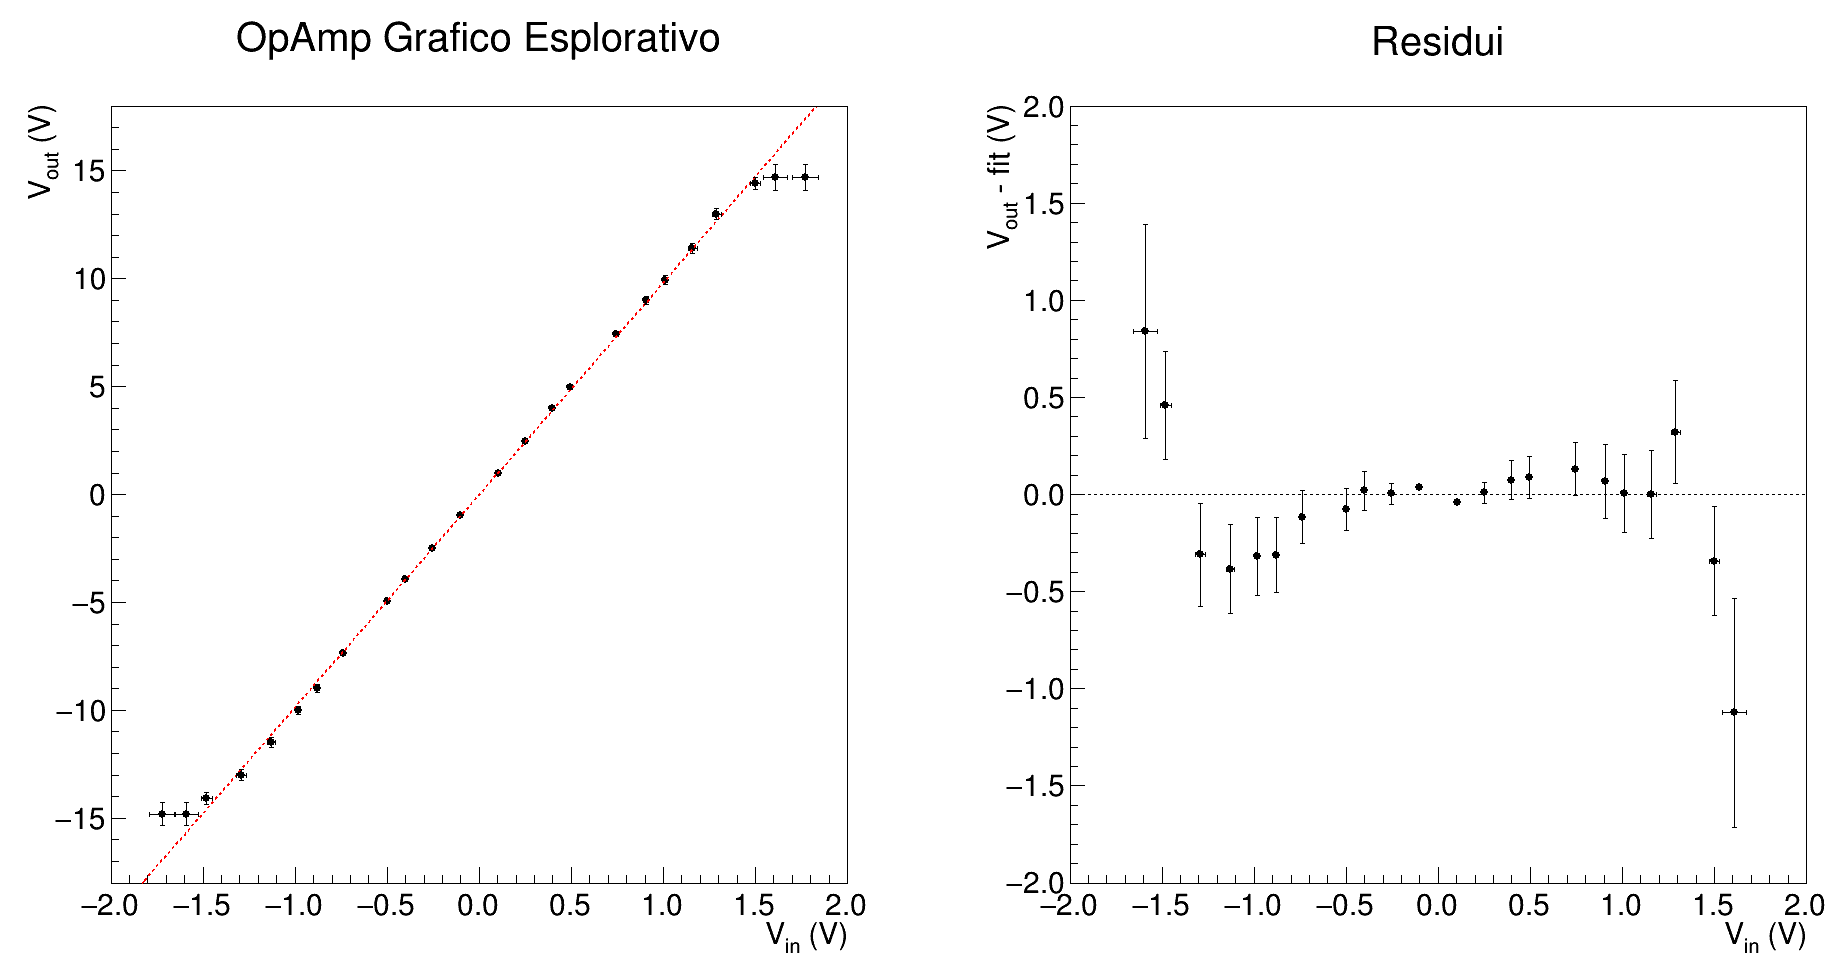
\includegraphics[width=\linewidth]{../Plots/Report_Plots/opamp_plot_alldata_eda.png}
	\caption{\small Grafico delle misure acquisite interpolate linearmente e relativo grafico dei residui.}
	\label{i:opamp_eda}
\end{figure}

\noindent  Si vuole inizialmente far notare che i valori di $V_{\text{in}}$ sono conformi a quanto impostato sul
generatore: questo è sicuramente indice di una corretta acquisizione del segnale in ingresso e di una corretta
configurazione del generatore (\textit{modalità "50 Ohm"}) e dell'oscilloscopio (\textit{attenuazione sonda 10X}).
Osservando invece i valori di $V_{\text{out}}$ si nota un'amplificazione conforme alle aspettative (circa un fattore
10). Inoltre si osserva come le ultime misure, cioè quelle con tensione nominale $V\text{pp}_{\text{gen}}$ maggiore,
tendano a stabilizzarsi attorno a circa $V_{\text{sat}}=\pm15\,\si{\volt}$, ovvero la tensione massima che
l'amplificatore operazionale può fornire in output. Come da aspettative, riportate in \autoref{s:spice}, questo fenomeno
di stabilizzazione attorno a $V_{\text{sat}}$ inizia a manifestarsi attorno ad una tensione erogata dal generatore di
circa $V\text{pp}_{\text{gen}}=3\,\si{\volt}$. Dal grafico dei residui si può osservare lo stesso fenomeno: la zona
centrale risulta essere distribuita ragionevolmente attorno allo zero, mentre gli estremi tendono a distanziarsi anche
notevolmente. Da questo si deduce dunque che i tre punti finali di massimo e di minimo sono da considerarsi degli
outliers rispetto al trend lineare delle misure rimanenti: al fine di caratterizzare la linearità dell'amplificatore
operazionale e di calcolare l'amplificazione del circuito, dunque, gli outliers non verranno considerati.

%----------------------------------------------------------------------------------------
%	PRELIMIARY FIT
%----------------------------------------------------------------------------------------

\subsubsection{Interpolazioni Preliminari}\label{s:pre} Si procede ora considerando il campione di misure dei massimi ed
il campione di misure dei minimi separatamente, in quanto a priori non si ha la certezza che queste risentano della
stessa amplificazione e che non sia presente una sistematica di offset/shift verticale tra i due dataset. Si cercherà in
seguito di caratterizzare l'accordo tra i due dataset studiando la compatibilità tra i coefficienti angolari e tra le
intercette della retta interpolante. Osservando le misure in  \autoref{i:opamp_eda} si nota come le incertezze su
$V_{\text{in}}$ siano generalmente un ordine di grandezza inferiori rispetto a quelle su $V_{\text{out}}$: le prime non
sono quindi trascurabili rispetto alle seconde. Per tenere conto dell'incertezza su $V_{\text{in}}$, ci si propone
allora di effettuare un fit preliminare, nel quale si considerano unicamente gli errori su $V_{\text{out}}$, per stimare
un coefficiente angolare $m$. Questo viene poi utilizzato per proiettare gli errori di $V_{\text{in}}$ lungo l'asse
delle ordinate secondo 

\begin{equation}\label{e:proj}
	\sigma_{y} = \sqrt{	\sigma_{V_{\text{out}}}^2	+	m^2	\sigma_{V_{\text{in}}}^2	}
\end{equation}

\noindent I coefficienti angolari di interesse sono dunque riportati in  \autoref{t:pre_slopes}.

\begin{table}[H]
	\small
	\centering
	\begin{tabular}{x{4cm} x{4cm}} 

		\toprule[0.5px]
		\toprule[0.1px]
		
		\multicolumn{2}{c}{Coefficienti Angolari Preliminari}\tn
		\midrule[0.1px]

		Campione di Massimi & Campione di Minimi \tn

		\addlinespace
		
		$m=10.02\pm0.09$ & $m=10.16\pm0.09$ \tn
		
		\bottomrule[0.5px]
		
	\end{tabular}
	\caption{\small Valori dei coefficienti angolari restituiti dalle interpolazioni preliminari.}
	\label{t:pre_slopes}
\end{table}	

%----------------------------------------------------------------------------------------
%	LINEARITA E AMPLIFICAZIONE
%----------------------------------------------------------------------------------------


\subsubsection{Linearità e Amplificazione}
Alla luce di quanto trovato nella sezione precedente, si ripetono le interpolazioni lineari associando ai punti un
errore dato da  \autoref{e:proj} ed i parametri restituiti dai fit sono riportati in  \autoref{t:opamp_fitres_max_min}.

\begin{table}[H]
	\centering
	\small
	\begin{tabular}{x{3cm} x{3cm} x{3cm} x{3cm}} 

		\toprule[0.5px]
		\toprule[0.1px]
		
		\multicolumn{4}{c}{Fit Parameters}\tn
		\midrule[0.1px]

		\multicolumn{4}{c}{Campione di Massimi}\tn

		\addlinespace
		
		Offset (V) & Slope & $\chi^2$/ndf & $\sigma_{\text{posteriori}}$ (V)\tn

		\addlinespace

		$-0.06\pm0.04$ & $10.02\pm0.14$ & $0.98/7$ & $0.10$ \tn

		\midrule[0.1px]
		
		\multicolumn{4}{c}{Campione di Minimi}\tn

		\addlinespace
		
		Offset (V) & Slope & $\chi^2$/ndf & $\sigma_{\text{posteriori}}$ (V) \tn

		$0.07\pm0.04$ & $10.16\pm0.14$ & $0.67/7$ & $0.07$ \tn



		\bottomrule[0.5px]
		
	\end{tabular}
	\caption{\small Parametri della retta interpolante, il valore del $\chi^2$ associato al fit 
	e l'errore a posteriori relativo alla distribuzione dei dati.}
	\label{t:opamp_fitres_max_min}
\end{table}	

\noindent Dai parametri presentati in  \autoref{t:opamp_fitres_max_min} si riescono ad estrarre numerose informazioni
riguardo ai due campioni di dati. Inizialmente, si vuole far notare come i due coefficienti angolari siano in ottima
compatibilità tra loro: $\lambda=0.7$. Da questo si può assumere che i due dataset risentano della stessa amplificazione
$G$, come da aspettative. Successivamente, si può notare invece che le due intercette delle rette interpolanti sono in
leggera compatibilità con lo zero ($\lambda \approx 1.5$), mentre tra loro presentano una compatibilità $\lambda=2.4$,
che fa sorgere l'idea di una possibile sistematica di offset/shift verticale tra i due dataset (computando la differenza tra le
due intercette si trova uno sfalsamento $d=0.13 \pm 0.05 \,\si{\volt}$). Osservando poi il valore del $\chi^2$, si
ritrova in per entrambi i campioni $\chi^2/\nu<1$ (con $\nu\equiv\text{ndf}$ il numero di gradi di libertà, che coincide
con il valore di aspettazione $E(\chi^2)$). Ricordando che le incertezze sul guadagno verticale dell'oscilloscopio sono
almeno parzialmente correlate, gli errori associati alle misure sono tra loro correlati: questo spiega i valori di
$\chi^2$ eccessivamente ridotti. Un'interpolazione di dati con incertezze correlate restituisce parametri con errori
sottostimati, in quanto il fit non tiene conto della correlazione tra incertezze delle misure. Si può dunque assumere
che i parametri \textit{slope} e \textit{offset} riportati in \autoref{t:opamp_fitres_max_min} presentino in realtà una
compatibilità maggiore, proprio a causa di una possibile sottostima dell'errore sui parametri. Si vuole allora assumere
che i due campioni risentano della stessa amplificazione e che non siano tra loro sfalsati verticalmente in modo
significativo: segue quindi un tentativo di "unificazione" del campione di dati ed un'interpolazione lineare unica che
tenga conto sia dei massimi che dei minimi. Il grafico rappresentante i due dataset unificati con relativa
interpolazione lineare è mostrato in \autoref{i:opamp_all_proj}. 
%----------------------------------------------------------------------------------------
%	FIT UNIFICATO
%----------------------------------------------------------------------------------------
\begin{figure}[H]
	\centering
	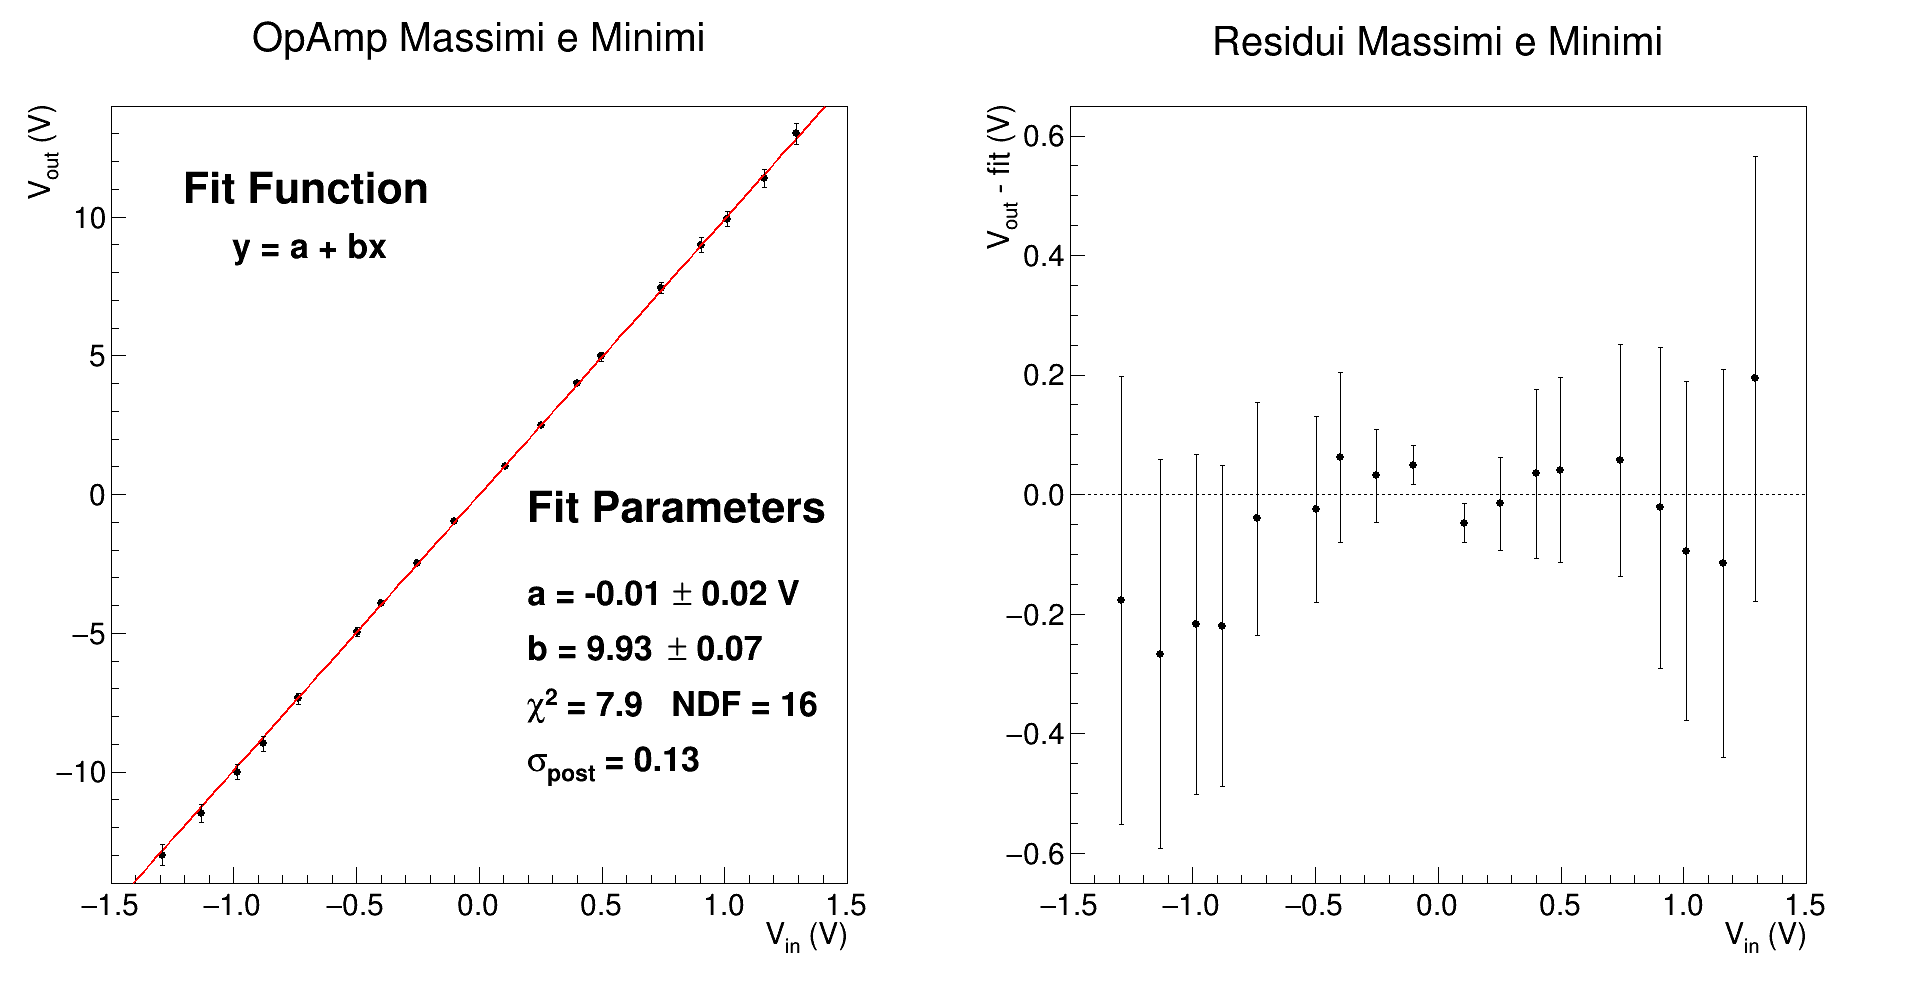
\includegraphics[width=\linewidth]{../Plots/Report_Plots/opamp_plot_all_projected.png}
	\caption{\small A sinistra: grafico rappresentante il dataset dei massimi ed il dataset dei minimi uniti assieme, 
	con relativa retta interpolante e parametri del fit. A destra: grafico dei residui $V_{\text{out}}-\text{fit}$.}
	\label{i:opamp_all_proj}
\end{figure}

\noindent Si osserva inizialmente che l'intercetta della retta interpolante è ora ben compatibile con zero, mentre il
coefficiente angolare presenta un errore relativo $\sigma_{b}/b=0.7\%$, che si può continuare ad assumere sottostimato:
la correlazione tra gli errori di scala, infatti, si può notare chiaramente dall'andamento "a farfalla" delle barre
d'errore nel grafico dei residui. Il valore del $\chi^2$ migliora leggermente rispetto alle interpolazioni dei dataset
separati: la compatibilità con il valore di aspettazione risulta essere $Z=1.4$. L'errore a posteriori, inoltre, si
trova in una zona intermedia rispetto alla gamma di errori associati alle misure: non potendo eliminare la correlazione
tra le incertezze si può affermare dunque che l'errore è in media stimato correttamente e l'oscilloscopio lavora entro
le specifiche. I residui, infatti, si posizionano tutti entro il loro errore, alcuni anche abbondantemente.
Focalizzandosi ora sulla stima del coefficiente angolare si nota che questo, $m=9.93\pm 0.07$, pur essendo ben
compatibile con i risultati esposti in  \autoref{t:opamp_fitres_max_min} relativi ai fit dei due campioni di misure
considerati separatamente, si trova essere sensibilmente minore di entrambi: ci si sarebbe aspettato, invece, di trovare
un valore intermedio unificando i due campioni di misure. Osservando poi il grafico dei residui, si può notare un
andamento leggermente anomalo, quasi parabolico, avente concavità rivolta verso il basso. Si ipotizza dunque che
l'assunzione fatta in precedenza riguardo la presenza di una sistematica di offset/shift verticale tra i due dataset
trascurabile necessiti di essere rivisitata. Per approfondire maggiormenta la questione, si decide di computare le
grandezze "picco picco" delle tensioni in ingresso $V_{\text{in}}$ e in uscita $V_{\text{out}}$ secondo
$V_{\text{pp}}=V^{\text{max}}-V^{\text{min}}$. Per quanto riguarda l'errore da associare alle grandezze picco picco, si
ricorda che l'oscilloscopio misura la differenza $\Delta$ tra i due cursori con una precisione ancora maggiore rispetto
alla singola misura. Si decide dunque di non aggiungere il fattore moltiplicativo $\sqrt{2}$ alla propagazione
presentata in  \autoref{e:osc}, al fine di evitare sovrastime eccessive dell'errore. Si procede ora come mostrato in
\autoref{s:pre}, effettuando inizialmente un fit lineare preliminare considerando solo gli errori su $Vpp_{\text{out}}$
e, utilizzando il coefficiente angolare restituito da tale interpolazione, si prosegue proiettando gli errori secondo
\autoref{e:proj}. Si ripete quindi il fit, che viene rappresentato in \autoref{i:opamp_pp}. Osservando il grafico dei
residui, si nota immediatamente come ora l'andamento anomalo è del tutto assente ed i punti si distribuiscono in modo
ottimale attorno allo zero. Rimane, chiaramente, il tipico andamento crescente delle barre d'errore, indice che le
incertezze continuano a risentire della correlazione tra esse. Il valore del $\chi^2$ è decisamente basso rispetto al
numero di gradi di libertà, come suggerito dal grafico dei residui in cui si nota chiaramente come la distanza
punto-retta sia ampiamente compresa entro la barra d'errore del dato. L'errore a posteriori è appena maggiore
dell'incertezza associata al primo punto, mentre diventa notevolmente inferiore per i successivi.
%----------------------------------------------------------------------------------------
%	FIT PICCO PICCO
%----------------------------------------------------------------------------------------
\begin{figure}[H]
	\centering
	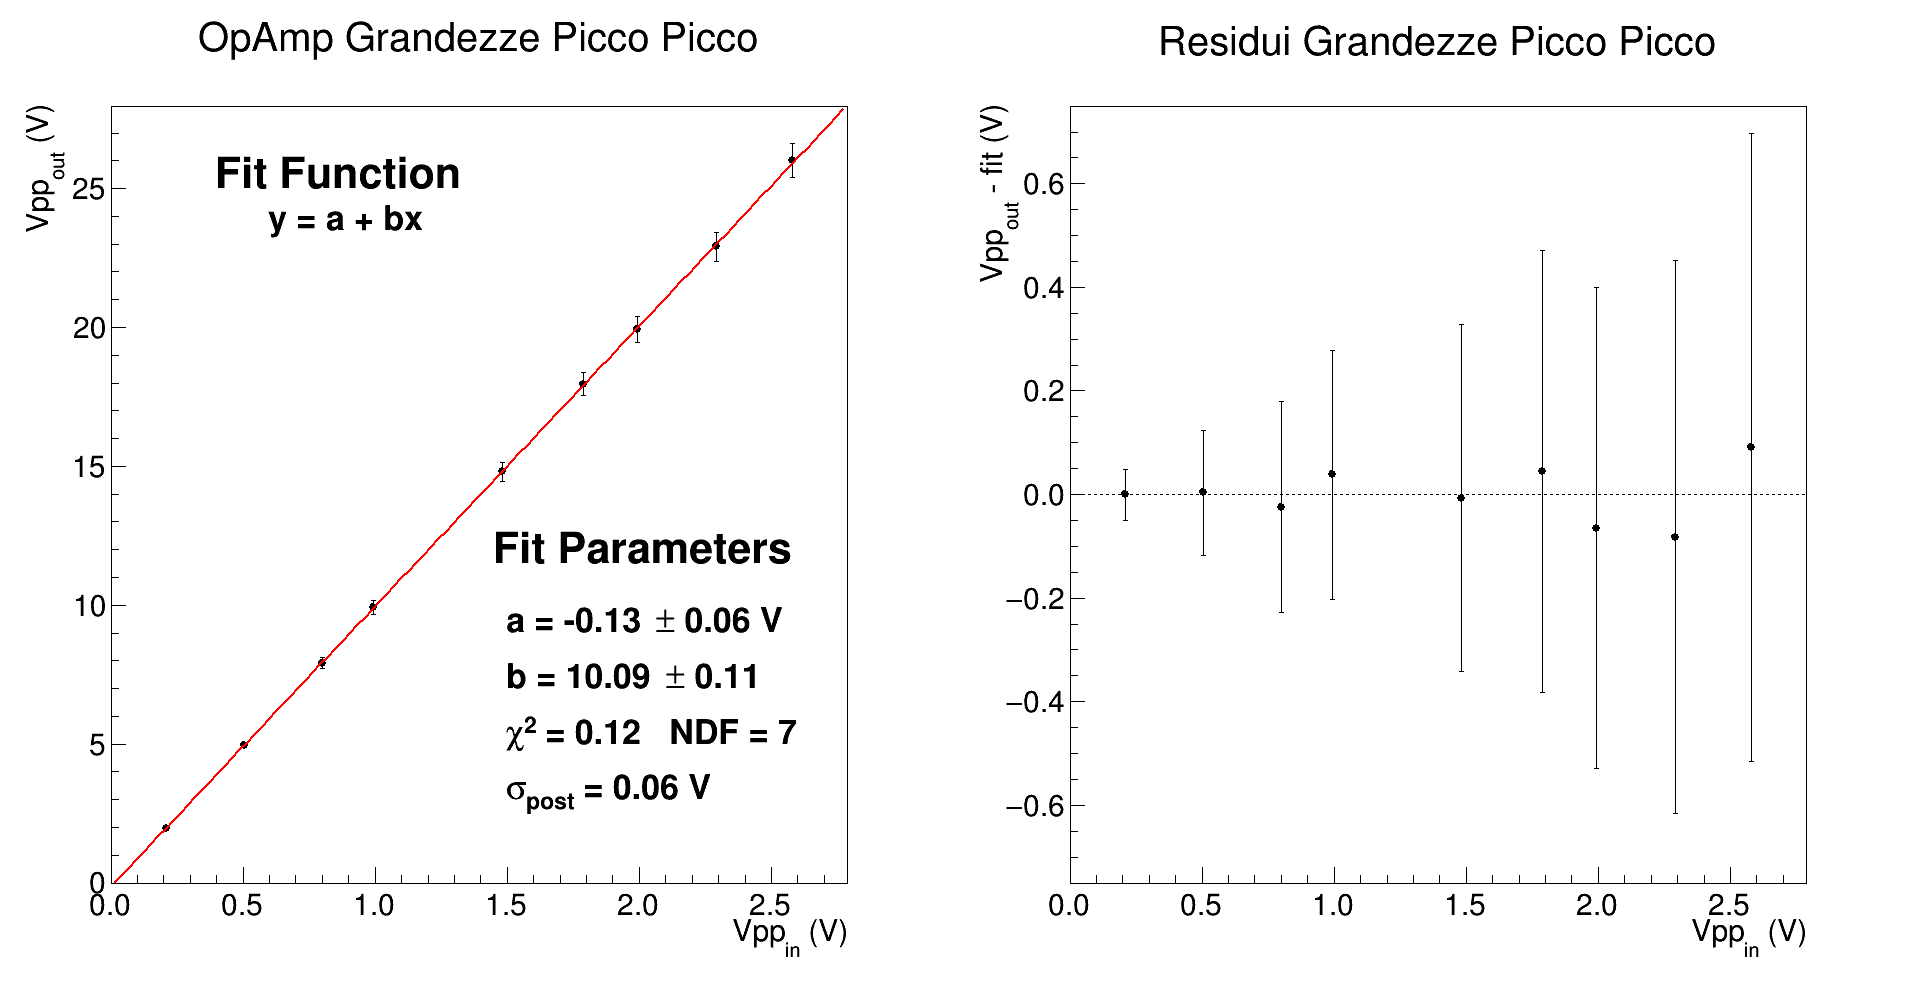
\includegraphics[width=\linewidth]{../Plots/Report_Plots/opamp_plot_pp_projected.png}
	\caption{\small A sinistra: grafico rappresentante il dataset delle grandezze picco picco, 
	con relativa retta interpolante e parametri del fit. A destra: grafico dei residui $V\text{pp}_{\text{out}}-\text{fit}$.}
	\label{i:opamp_pp}
\end{figure}

\noindent  Il valore dell'intercetta, scarsamente compatibile con lo zero, suggerisce una conferma all'ipotesi un una
sistematica di offset/shift verticale tra i due dataset non trascurabile. Il coefficiente angolare, invece, è
perfettamente in linea con i parametri ottenuti considerando i due dataset separatamente: calcolando la media pesata dei
due, infatti, si trova $\langle m\rangle_{\text{max, min}}=10.09 \pm 0.10$ e risulta avere una compatibilità
estremamente elevata con il coefficiente angolare riguardante il dataset delle grandezze picco picco ($\lambda = 0.01$).
Si assume dunque che questi due valori ($\langle m\rangle_{\text{max, min}}$ ed il coefficiente angolare del campione di
grandezze picco picco $m_{\text{pp}}$) rappresentino una soddisfacente stima dell'amplificazione \textit{G} del
circuito. Per quanto riguarda la linearità dell'amplificatore operazionale, invece, i valori estremamente ridotti del
$\chi^2$ non permettono nè di confermare l'ipotesi di linearità nè di poterla rigettare. Si ripone allora maggior
attenzione alla distribuzione delle misure attorno alla retta (o meglio alla distribuzione dei residui attorno allo
zero) che si ritiene invece, in questa occasione, determinante: il campione di misure picco picco suggerisce una
soddisfacente distribuzione lineare dei dati. 


%----------------------------------------------------------------------------------------
%	CONFRONTO STIME DI G
%----------------------------------------------------------------------------------------

\subsubsection{Confronto tra Stime di G}
 Si vuole ora esporre e confrontare le stime dell'amplificazione del circuito, rappresentando i valori del guadagno
\textit{G} in \autoref{i:opamp_comp}. Partendo dal primo punto a sinistra, cioè la stima di \textit{G} tramite le misure
dirette delle resistenze $R_{\text{f}}$ e $R_{1}$ (riportate in \autoref{t:direct_measures}), si nota come questo
presenti un errore 

\begin{wrapfigure}{L}{0.5\textwidth}
	\centering
	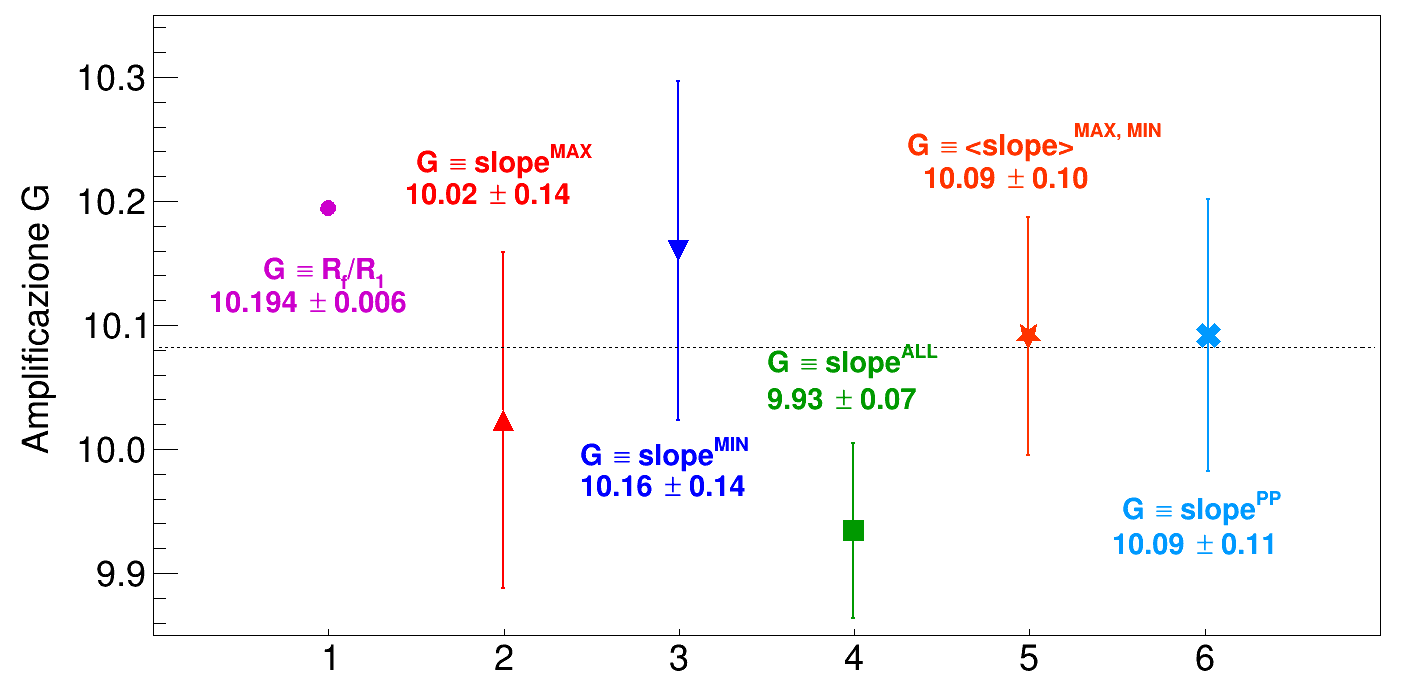
\includegraphics[width=0.5\textwidth]{../Plots/Report_Plots/opamp_comp_BIG.png}
	\caption{\footnotesize Stime di G. Da sinistra: 1) partendo dalle misure dirette delle resistenze; 2) come
	coefficiente angolare del dataset di massimi; 3) come coefficiente angolare del dataset di minimi; 4) come
	coefficiente angolare del dataset unificato; 5) come media pesata di 2 e 3; 6) come coefficiente angolare del
	dataset delle grandezze picco picco.}
	\label{i:opamp_comp}
\end{wrapfigure}

\noindent nettamente inferiore a confronto con le rimanenti stime. Quest'ultime risultano essere quantità compatibili
con 1) $G=R_{\text{f}}/R_{1}$, ad eccezione di 4) quella ottenuta considerando assieme sia i massimi sia i minimi
($\lambda = 3.7$). In particolare, si può osservare come la media pesata 5) tra le stime dell'amplificazione ottenute
considerando i campioni separati e la stima ottenuta con le grandezze picco picco 6) si trovino in eccellente accordo:
si può concludere dunque che, eliminando la sistematica di offset/shift verticale tra i due dataset (sia attraverso
grandezze picco picco, sia considerando la media pesata dei risultati ottenuti dai campioni separati), la stima
dell'amplificazione del circuito risulta essere compatibile con le aspettative preliminari. Si assume in ogni caso che
l'errore su \textit{G} sia sottostimato a causa della correlazione delle incertezze: si preferisce dunque la stima
ritrovata considerando le tensioni picco picco 6), in quanto presenta un errore relativo leggermente maggiore.


%----------------------------------------------------------------------------------------
%	CIRCUITO DERIVATORE
%----------------------------------------------------------------------------------------

\section{Filtro Attivo - Circuito Derivatore}
Ci si propone di studiare il comportamento \textit{in frequenza} di un circuito simile a quello
considerato in \autoref{s:opamp}, con l'aggiunta di un condensatore $C_{1}$ in serie alla resistenza $R_{1}$: questo lo
rende dunque un filtro (attivo, in quanto è sempre presente l'amplificatore operazionale) passa alto, derivatore a basse
frequenze. 

%----------------------------------------------------------------------------------------
%	CONFIGURAZIONE SPERIMENTALE
%----------------------------------------------------------------------------------------

\subsection{Configurazione Sperimentale}
Utilizzando la stessa configurazione circuitale rappresentata in \autoref{i:opamp_circuit}, viene aggiunta la capacità
$C_{1} = 0.977 \pm 0.017 \,\si{n\farad}$ (misurata direttamente utilizzando il multimetro digitale a fondo scala
$1\,\si{n\farad}$) in serie alla resistenza $R_{1}$, tra essa e l'amplificatore operazionale. Nel dominio delle
frequenze la funzione di trasferimento $H(s)=V_{\text{out}}(s)/V_{\text{in}}(s)$ del circuito risulta essere 
\begin{align}
	H(s) &= -\frac{R_{\text{f}}}{R_{1}}\frac{s}{s+\omega_{0}} & \text{con}\,\,\,\, \omega_{0}&=\frac{1}{R_{1}C_{1}}
\end{align}

\noindent Si nota dunque che il termine $-\frac{R_{\text{f}}}{R_{1}}$ è esattamente il guadagno $G$ (il segno meno è
sempre legato al fatto che l'operazionale è posto in configurazione invertente) del circuito studiato in
\autoref{s:opamp}, mentre il termine $\frac{s}{s+\omega_{0}}$ risulta essere analogo alla funzione di trasferimento di
un circuito passa alto passivo. Ci si aspetta dunque che a basse frequenze il circuito si comporti come un derivatore,
mentre, essendo un passa alto, ci si aspetta si ottenga il massimo guadagno per $s\rightarrow\infty$ e che questo sia
esattamente $G$. Si imposta allora il generatore in modo da erogare un'onda sinusoidale di ampiezza $1\,\si{\volt}$
picco picco (che verrà mantenuta costante) e frequenza variabile tra $100\,\si{\Hz}$ e $1\,\si{\MHz}$ per lo studio
della risposta in frequenza del circuito. Avendo misurato le componenti circuitali direttamente con i multimetri, la
stima attesa del massimo guadagno è già stata esplicitata in \autoref{e:guadagno}, mentre ci si aspetta una frequenza di
taglio

\begin{align}
	f_{\text{t}}&=20.1 \,\si{k\Hz} & \sigma_{f_{\text{t}}}&=\sqrt{	\left(\frac{1}{C_{1}R_{1}^2}\right)^2\sigma_{R_{1}}^2	+
																	\left(\frac{1}{C_{1}^2R_{1}}\right)^2\sigma_{C_{1}}^2   }
																	= 0.3 \,\si{k\Hz}	
\end{align}


%----------------------------------------------------------------------------------------
%	ACQUISIZIONE MISURE
%----------------------------------------------------------------------------------------

\subsection{Acquisizione Misure}
Per studiare la risposta in frequenza del circuito, si fa variare la frequenza del segnale in ingresso da
$100\,\si{\Hz}$ a $1\,\si{\MHz}$ e vengono acquisite misure di tensione picco picco sia del segnale in ingresso sia di
quello in uscita: inizialmente viene effettuata un'acquisizione preliminare con il fine di individuare gli intervalli di
frequenze più interessanti, quali l'intorno della frequenza di taglio e l'intorno del massimo di amplificazione (si
trova infatti che questo non viene assunto al tendere della frequenza verso valori sempre maggiori, ma piuttosto si ha
un fenomeno di attenuamento di amplificazione oltre un certo range di frequenze). Così facendo, si riesce a fornire una
stima approssimativa della frequenza di taglio. Infatti, infittendo le misure in tali intervalli si trova
l'amplificazione massima sperimentale ($G_{\text{sper}}\approx 9.8$): questa viene divisa per un fattore $\sqrt{2}$ e,
successivamente, si ricerca la frequenza che corrisponde a tale amplificazione ridotta, sempre infittendo le misure
nell'intorno della frequenza di taglio. Si trova quindi $f_{\text{t, sper}}\approx 19.5\,\si{k\Hz}$.


%----------------------------------------------------------------------------------------
%	DATI E ANALISI
%----------------------------------------------------------------------------------------

\subsection{Dati e Analisi}
In questa sezione si vuole studiare il grafico di Bode relativo alle misure acquisite sperimentalmente sia con il fine di estrarre
informazioni di carattere generale sui dati, sia per fornire una stima della frequenza di taglio attraverso
l'interpolazione delle misure.


%----------------------------------------------------------------------------------------
%	THEBODE
%----------------------------------------------------------------------------------------

\subsubsection{Grafico di Bode}
Date le misure di tensione $V_{\text{in}}$ e $V_{\text{out}}$, viene calcolata la funzione di trasferimento
\begin{align}
	H&=\frac{V_{\text{out}}}{V_{\text{in}}} & \sigma_{H}&= H \sqrt{	
											\left(	\frac{	\sigma_{l}\times V_{\text{in}}/\text{div}	}{	V_{\text{in}}	}	\right)^2	 + 
											\left(	\frac{	\sigma_{l}\times V_{\text{out}}/\text{div}	}{	V_{\text{out}}	}	\right)^2 +	
											2\left(	\frac{	\sigma_{k}	}{	k	}	\right)^2 }	
\end{align}
\noindent dove $\sigma_{l}=0.04$ rappresenta l'incertezza di lettura associata all'oscilloscopio, i termini
$V_{\text{in}}/\text{div}$ e $V_{\text{out}}/\text{div}$ corrispondono al numero di volt per divisione per il canale di
acquisizione rispettivamente del segnale in ingresso e del segnale in uscita, mentre $\sigma_{k}=1.5\%$ rappresenta
l'incertezza di guadagno associata all'oscilloscopio: quest'ultima viene considerata in quanto le misure non sono state
acquisite utilizzando un'unica scala e, inoltre, sono state acquisite utilizzando due diversi canali. Si assume che $k$
sia mediamente pari all'unità. L'incertezza sulla frequenza dell'onda erogata dal generatore si assume trascurabile. Si
rappresenta allora in \autoref{i:diff_bode} il grafico di Bode delle misure acquisite assieme ai punti simulati con
LTSpice. Osservando il grafico si nota che sono state effettuate due interpolazioni: la prima lineare, per la quale sono
state considerate le prime tre misure, mentre la seconda parabolica, per la quale sono state considerate le misure
nell'intorno del massimo di amplificazione. La strategia per stimare la frequenza di taglio è la seguente: si stima il
massimo della funzione di trasferimento come vertice della parabola, si considera quindi la retta orizzontale
$y=H_{\text{max}}$ e si calcola il punto di intersezione con la retta $y=a+bx$ interpolante le prime tre misure
crescenti. In questo modo, la coordinata $x$ del punto di intersezione coincide con la frequenza di taglio del circuito.
Prima di discutere la frequenza di taglio del circuito, tuttavia, si vogliono fare delle considerazioni di carattere più
generale sul campione di dati rappresentato in \autoref{i:diff_bode}. Per la parte lineare (a sinistra) si può notare un
soddisfacente accordo tra misure sperimentali e dati simulati, e lo stesso vale nell'intorno della frequenza di taglio e
nell'intorno del massimo della funzione di trasferimento. Per questo motivo si può affermare che, siccome nell'analisi
per la ricerca della frequenza di taglio vengono utilizzate le misure che sono in accordo con le aspettative, i
risultati sono da considerarsi significativi. Si nota tuttavia che la retta presenta un coefficiente angolare ($b =
19.03\pm 0.16\,\text{dB/dec}$ leggermente minore a confronto con le aspettative teoriche ($b_{\text{th}}=20\,\text{dB/dec}$)


\begin{figure}[H]
	\centering
	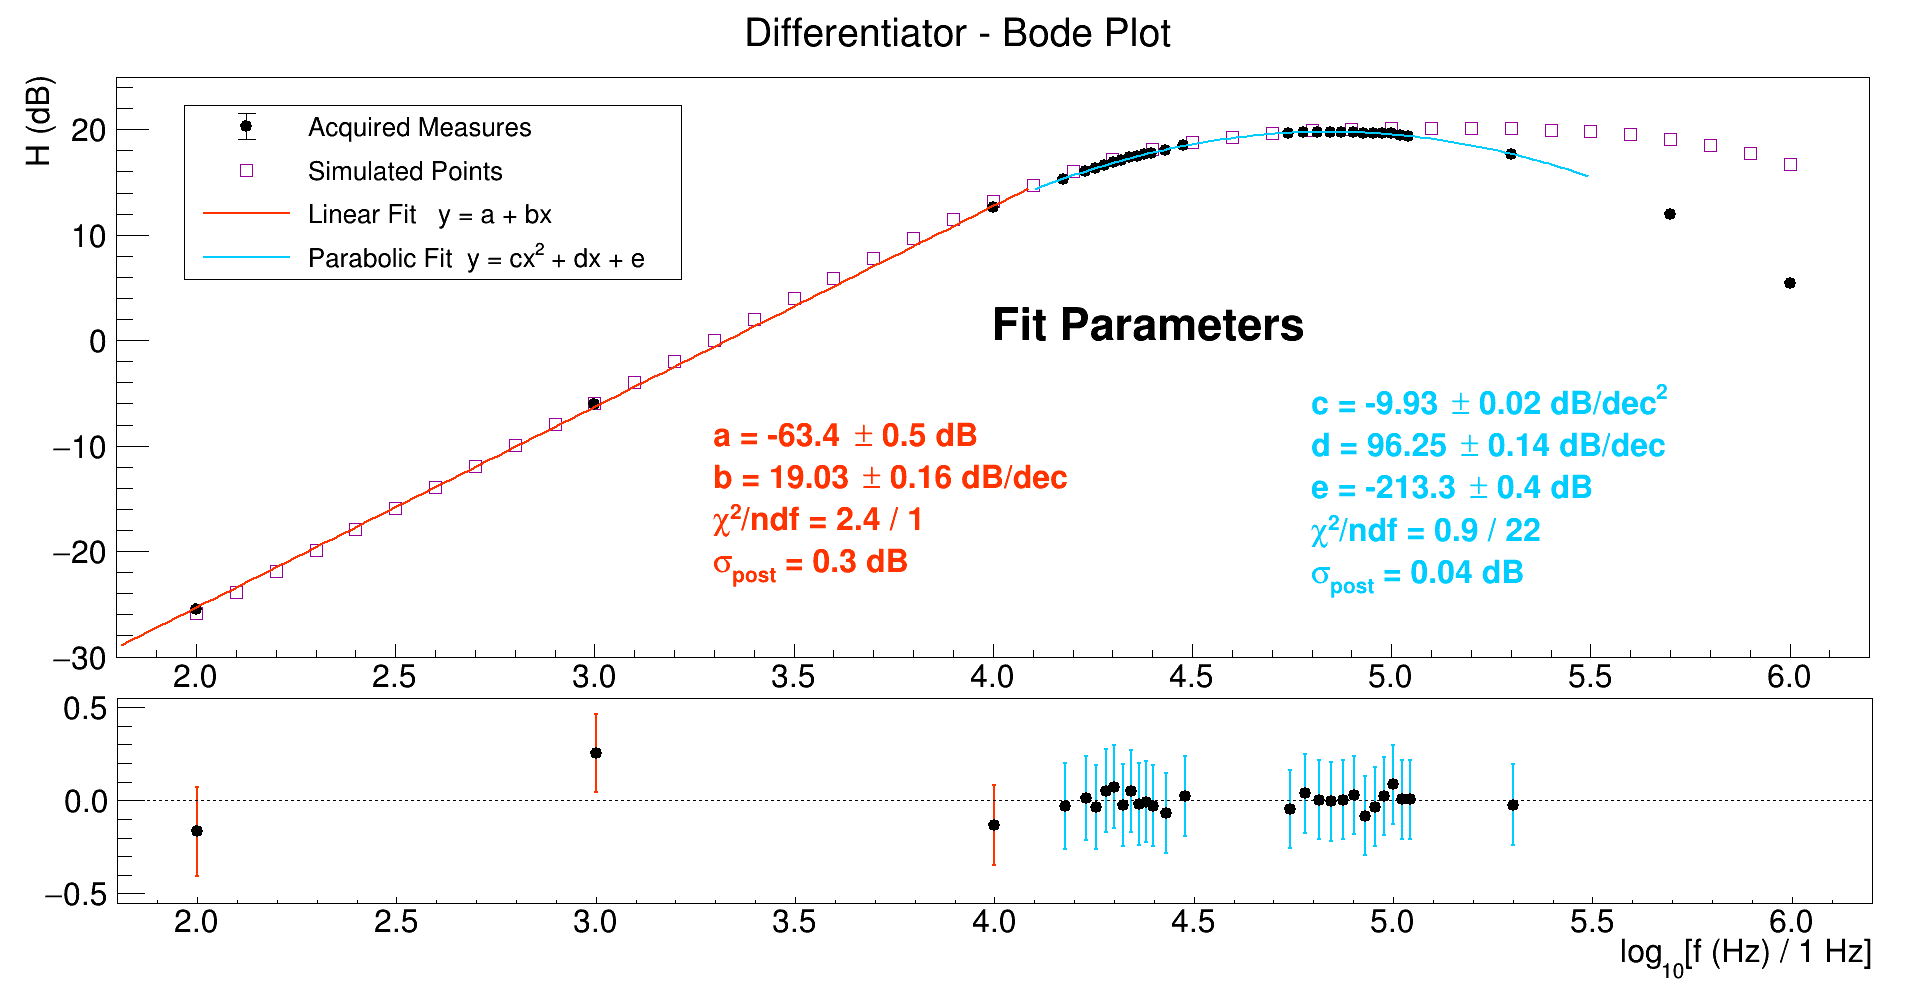
\includegraphics[width=\linewidth]{../Plots/Report_Plots/diff_bode.png}
	\caption{\small Grafico di Bode delle misure sperimentali e dei dati simulati. Le misure sperimentali vengono
	interpolate con una retta $y = a + bx$ e con una parabola $y = cx^2+dx+e$. Vengono mostrati anche i residui, 
	rispettivamente per la retta e per la parabola.}
	\label{i:diff_bode}
\end{figure}








































\cleardoublepage
%----------------------------------------------------------------------------------------
%	ARDUINO
%----------------------------------------------------------------------------------------
\cleardoublepage
\section{Arduino}
In questa sezione si vuole effettuare una calibrazione della scheda Arduino Due. In particolare, si vuole quantificare
il sampling rate dell'ADC della scheda e determinare la funzione di calibrazione in tensione, ovvero $V = a
+ b \cdot \text{ADC}$ dove $V$ è il valore in Volt del segnale, $\text{ADC}$ è la tensione in ADC counts acquisita da
Arduino, mentre $a$ e $b$ sono i parametri di calibrazione. 

%----------------------------------------------------------------------------------------
%	SAMPLING RATE 
%----------------------------------------------------------------------------------------

\subsection{Sampling Rate}
Si comincia configurando il segnale di trigger. Si imposta quindi nel canale CH2 del generatore un impulso quadrato di
durata $10\,\si{\us}$, frequenza $1\,\si{k\hertz}$ e altezza $2\,\si{\volt}$ a partire dallo zero. Sul canale CH1 del
generatore, invece, si imposta un'onda quadra di ampiezza $1\,\si{\volt}$ partendo da zero con frequenza
$5\,\si{k\hertz}$. Conoscendo il periodo dell'onda quadra in ingresso ($T=1/f$), il sampling rate viene computato come
$S = N / T = N \, f$ con $N$ il numero di misure acquisite in un periodo. Per calcolare $N$ viene computata la derivata
numerica della forma d'onda: questa presenterà dei picchi positivi quando la funzione passa da zero a $1\,\si{\volt}$ e
picchi negativi quando scende da $1\,\si{\volt}$ a zero. Il numero di acquisizioni in un periodo sarà allora il numeri
di punti compresi tra due picchi positivi della funzione derivata. Si trova allora un sampling rate $S = 955000 s^{-1}$,
ovvero 955000 acquisizioni al secondo.


%----------------------------------------------------------------------------------------
%	CALIBRAZIONE IN TENSIONE
%----------------------------------------------------------------------------------------

\subsection{Calibrazione in Tensione}
Si vuole ora verificare la linearità dell'ADC interno alla scheda e stimare i parametri $a$, $b$ della funzione di
calibrazione, in quanto si è interessati a convertire il segnale acquisito da ADC counts in Volt. Si acquisiscono allora
diverse forme d'onda facendo variare la tensione del generatore, avendo cura di misurare il segnale erogato con i
cursori dell'oscilloscopio, in quanto può non essere esattamente uguale a quello nominale indicato dal generatore. Si
rappresentano in grafico i valori di tensione $V$ misurati sperimentalmente contro la media dei punti appartenenti ai
picchi della relativa forma d'onda (si decide di non considerare unicamente il massimo della forma in quanto è possibile
si tratti di una fluttuazione). Effettuando poi un'interpolazione lineare si ricavano l'offset (cioè
quanti Volt corrispondono allo zero dell'ADC) ed il coefficiente angolare (cioè come scalano i Volt rispetto all'ADC).

\begin{figure}[H]
	\centering
	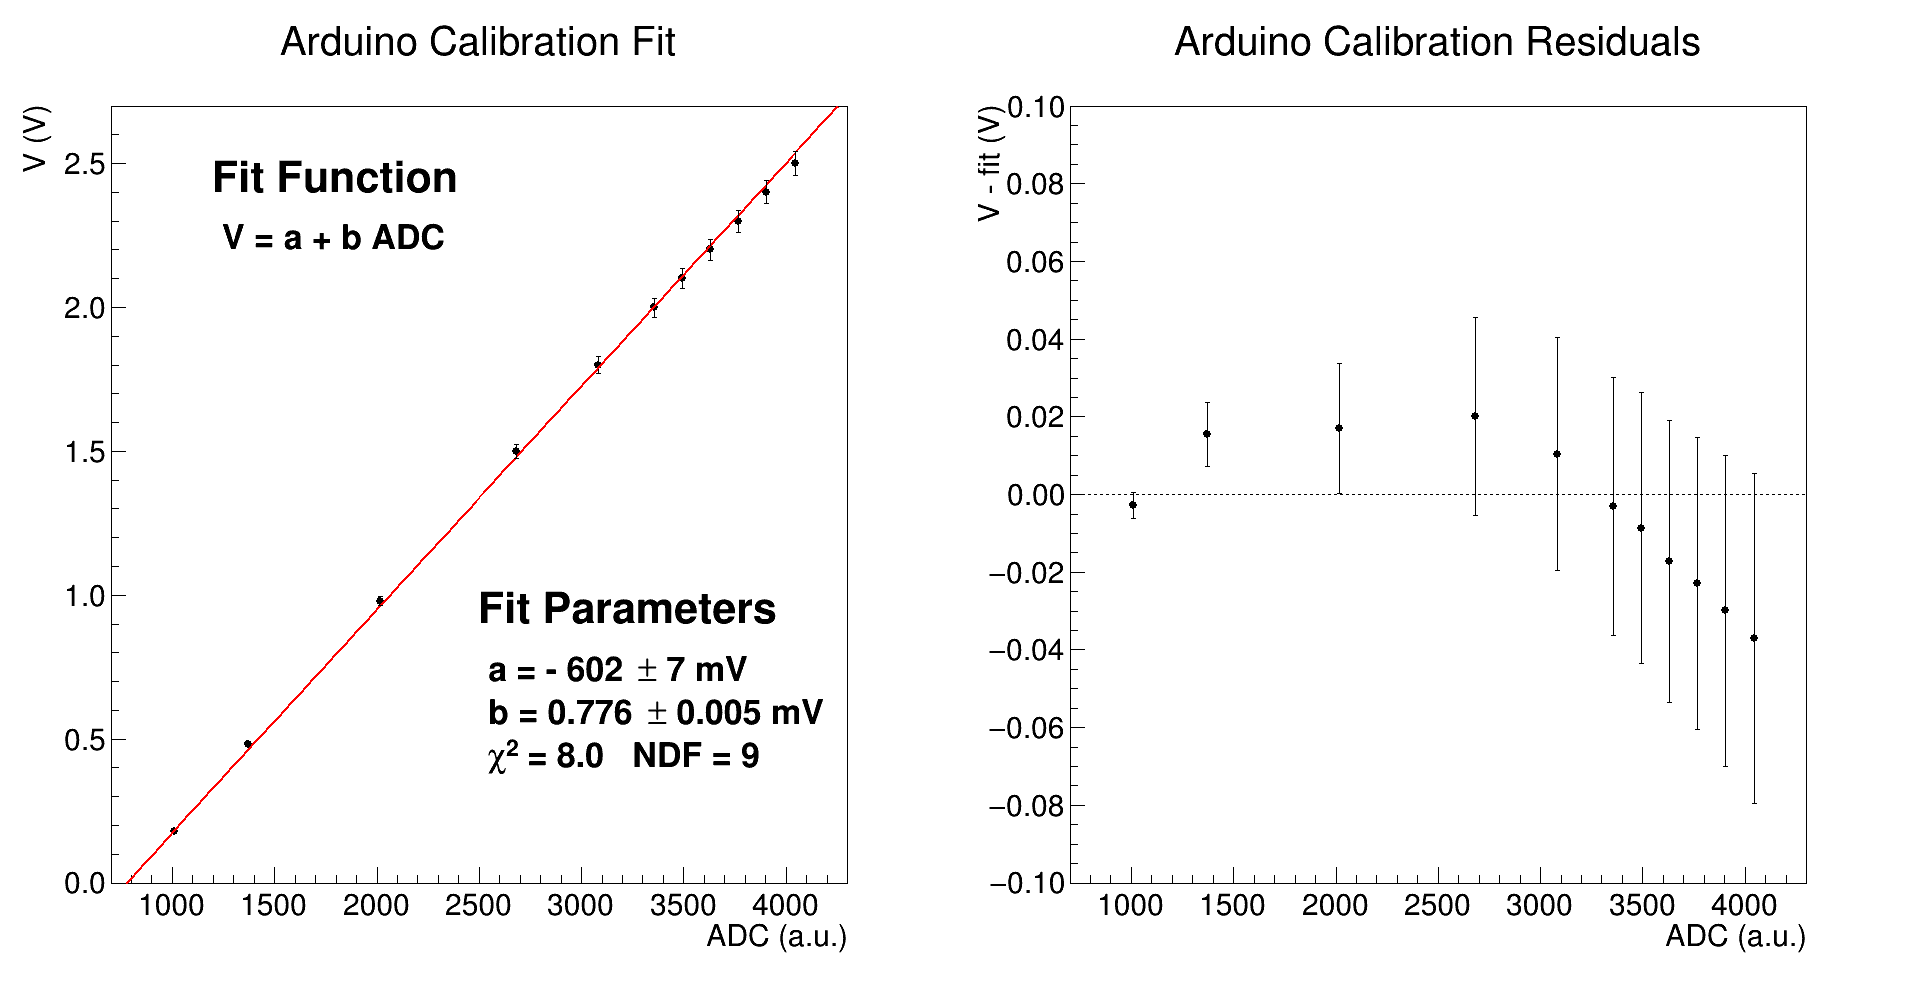
\includegraphics[width=\linewidth]{../Arduino/Plots/calib_function.png}
	\caption{Grafico di calibrazione in tensione e relativo grafico dei residui.}
	\label{i:ar_calib}
\end{figure}

\noindent Osservando il grafico dei residui, si nota un marcato andamento anomalo dei punti a tensioni maggiori, oltre i
$2\,\si{\volt}$: la scheda, cioè, risponde in modo leggermente diverso a seconda della tensione in ingresso. Questo è,
molto probabilmente, dovuto al circuito di protezione dei pin di ingresso (limitatore di tensione a diodi, utile per
evitare di bruciare la scheda) che ne altera la risposta avvicinandosi a tensioni pericolose. Si prova allora ad
effettuare nuovamente l'interpolazione rimuovendo i punti relativi a tensioni in ingresso maggiori di $2\,\si{\volt}$:
nonostante l'andamento dei residui migliori, anche il primo punto (tensione in ingresso pari a $200\,\si{\mV}$) si trova
essere fuori trend. Si ottengono quindi due zone in cui la linearità dell'ADC risulta essere ottimale: la prima tra
$500\,\si{\mV}$ e $1.8\,\si{\volt}$ (parametri di calibrazione: $a = -0.59 \pm 0.02 \, \si{\V}$ e $b = 0.776 \pm 0.013
\,\si{\mV}/\text{a.u.}$) mentre la seconda tra $1.8\,\si{\volt}$ e $2.5\,\si{\volt}$ (parametri di calibrazione: $a =
-0.44 \pm 0.15 \, \si{\V}$ e $b = 0.73 \pm 0.04 \,\si{\mV}/\text{a.u.}$).



%----------------------------------------------------------------------------------------
%	CONCLUSIONI
%----------------------------------------------------------------------------------------

\section{Conclusioni}

\end{document}